\documentclass{beamer}\usepackage[]{graphicx}\usepackage[]{color}
%% maxwidth is the original width if it is less than linewidth
%% otherwise use linewidth (to make sure the graphics do not exceed the margin)
\makeatletter
\def\maxwidth{ %
  \ifdim\Gin@nat@width>\linewidth
    \linewidth
  \else
    \Gin@nat@width
  \fi
}
\makeatother

\definecolor{fgcolor}{rgb}{0.345, 0.345, 0.345}
\newcommand{\hlnum}[1]{\textcolor[rgb]{0.686,0.059,0.569}{#1}}%
\newcommand{\hlstr}[1]{\textcolor[rgb]{0.192,0.494,0.8}{#1}}%
\newcommand{\hlcom}[1]{\textcolor[rgb]{0.678,0.584,0.686}{\textit{#1}}}%
\newcommand{\hlopt}[1]{\textcolor[rgb]{0,0,0}{#1}}%
\newcommand{\hlstd}[1]{\textcolor[rgb]{0.345,0.345,0.345}{#1}}%
\newcommand{\hlkwa}[1]{\textcolor[rgb]{0.161,0.373,0.58}{\textbf{#1}}}%
\newcommand{\hlkwb}[1]{\textcolor[rgb]{0.69,0.353,0.396}{#1}}%
\newcommand{\hlkwc}[1]{\textcolor[rgb]{0.333,0.667,0.333}{#1}}%
\newcommand{\hlkwd}[1]{\textcolor[rgb]{0.737,0.353,0.396}{\textbf{#1}}}%

\usepackage{framed}
\makeatletter
\newenvironment{kframe}{%
 \def\at@end@of@kframe{}%
 \ifinner\ifhmode%
  \def\at@end@of@kframe{\end{minipage}}%
  \begin{minipage}{\columnwidth}%
 \fi\fi%
 \def\FrameCommand##1{\hskip\@totalleftmargin \hskip-\fboxsep
 \colorbox{shadecolor}{##1}\hskip-\fboxsep
     % There is no \\@totalrightmargin, so:
     \hskip-\linewidth \hskip-\@totalleftmargin \hskip\columnwidth}%
 \MakeFramed {\advance\hsize-\width
   \@totalleftmargin\z@ \linewidth\hsize
   \@setminipage}}%
 {\par\unskip\endMakeFramed%
 \at@end@of@kframe}
\makeatother

\definecolor{shadecolor}{rgb}{.97, .97, .97}
\definecolor{messagecolor}{rgb}{0, 0, 0}
\definecolor{warningcolor}{rgb}{1, 0, 1}
\definecolor{errorcolor}{rgb}{1, 0, 0}
\newenvironment{knitrout}{}{} % an empty environment to be redefined in TeX

\usepackage{alltt} 
% \usepackage{graphicx}
\usepackage{graphics}
\usepackage[T1]{fontenc}
\usepackage{verbatim}
\usepackage{etoolbox}
\usepackage{hyperref}
\makeatletter
\preto{\@verbatim}{\topsep=-6pt \partopsep=-6pt }
\makeatother
%\usepackage{fix-cm}
\setbeamercovered{transparent}


\renewcommand{\ni}{\noindent}


% \SweaveOpts{cache=TRUE, background="white"}


\title[2-Graphics]{2 - Advanced Graphics in R}
\subtitle{04 - Dates, Times, and Groups}
\date{\hspace{1in}}
\institute[ISU]{Iowa State University}
\IfFileExists{upquote.sty}{\usepackage{upquote}}{}
\begin{document}

\begin{frame}
\maketitle
\end{frame}



\begin{frame}
\frametitle{Outline}
\begin{itemize}
\item Dates and Times
\item \texttt{lubridate} package
\end{itemize}
\end{frame}


\begin{frame}
\frametitle{Dates and Times}
\begin{itemize}
\item Dates and times are deceptively tricky to work with\medskip
\item Formats - 02/05/2012 is February 5 or May 2? \medskip
\item Time Zones\medskip
\item POSIXct and POSIXlt format in R is difficult to work with
\end{itemize}
\end{frame}

\begin{frame}
\frametitle{\texttt{lubridate} package}
\begin{itemize}
\item available from CRAN (\texttt{install.packages("lubridate")})\medskip
\item Written by Garett Grolemund and Hadley Wickham\medskip
\item associated paper\\\emph{JSS: Dates and Times made easy with lubridate}\\\url{http://www.jstatsoft.org/v40/i03/paper
}
\end{itemize}
\end{frame}

\begin{frame}[fragile]
\frametitle{Instants of time}
\begin{itemize}
\item one moment in time, usually named, e.g. 
\begin{knitrout}\footnotesize
\definecolor{shadecolor}{rgb}{1, 1, 1}\color{fgcolor}\begin{kframe}
\begin{alltt}
\hlkwd{now}\hlstd{()}
\end{alltt}
\begin{verbatim}
## [1] "2014-10-01 15:54:36 CDT"
\end{verbatim}
\end{kframe}
\end{knitrout}
\item lubridate turns strings into instants with functions that have y, m, and d in their names
\begin{knitrout}\footnotesize
\definecolor{shadecolor}{rgb}{1, 1, 1}\color{fgcolor}\begin{kframe}
\begin{alltt}
\hlkwd{ymd}\hlstd{(}\hlstr{"2013-05-14"}\hlstd{)}
\end{alltt}
\begin{verbatim}
## [1] "2013-05-14 UTC"
\end{verbatim}
\begin{alltt}
\hlkwd{mdy}\hlstd{(}\hlstr{"05/14/2013"}\hlstd{)}
\end{alltt}
\begin{verbatim}
## [1] "2013-05-14 UTC"
\end{verbatim}
\begin{alltt}
\hlkwd{dmy}\hlstd{(}\hlstr{"14052013"}\hlstd{)}
\end{alltt}
\begin{verbatim}
## [1] "2013-05-14 UTC"
\end{verbatim}
\begin{alltt}
\hlkwd{ymd_hms}\hlstd{(}\hlstr{"2013:05:14 14:50:30"}\hlstd{)}
\end{alltt}
\begin{verbatim}
## [1] "2013-05-14 14:50:30 UTC"
\end{verbatim}
\end{kframe}
\end{knitrout}
\item Order matters!
\end{itemize}
\end{frame}

\begin{frame}
\frametitle{Your Turn}
\begin{itemize}
\item The data set \href{http://www.hofroe.net/R\%20workshops/02-r-graphics/data/05-data/chicago.csv}{chicago.csv} contains records for every flight departing from Chicago O'Hare in June 2008\medskip
\item Parse the Date variable into a Date-Time Object
\end{itemize}
\end{frame}

\begin{frame}[fragile]
\frametitle{Working with instants}
\begin{itemize}
\item Standard arithmetic operations now work on dates:
\begin{knitrout}\footnotesize
\definecolor{shadecolor}{rgb}{1, 1, 1}\color{fgcolor}\begin{kframe}
\begin{alltt}
\hlkwd{now}\hlstd{()} \hlopt{>} \hlkwd{ymd}\hlstd{(}\hlstr{"1970-01-01"}\hlstd{)}
\end{alltt}
\begin{verbatim}
## [1] TRUE
\end{verbatim}
\begin{alltt}
\hlkwd{now}\hlstd{()} \hlopt{-} \hlkwd{ymd}\hlstd{(}\hlstr{"1970-01-01"}\hlstd{)}
\end{alltt}
\begin{verbatim}
## Time difference of 16345 days
\end{verbatim}
\end{kframe}
\end{knitrout}
\item functions for extracting pieces of dates:
\begin{knitrout}\footnotesize
\definecolor{shadecolor}{rgb}{1, 1, 1}\color{fgcolor}\begin{kframe}
\begin{alltt}
\hlkwd{month}\hlstd{(}\hlkwd{now}\hlstd{())}
\end{alltt}
\begin{verbatim}
## [1] 10
\end{verbatim}
\begin{alltt}
\hlkwd{wday}\hlstd{(}\hlkwd{now}\hlstd{())}
\end{alltt}
\begin{verbatim}
## [1] 4
\end{verbatim}
\begin{alltt}
\hlkwd{wday}\hlstd{(}\hlkwd{now}\hlstd{(),} \hlkwc{label}\hlstd{=}\hlnum{TRUE}\hlstd{)}
\end{alltt}
\begin{verbatim}
## [1] Wed
## 7 Levels: Sun < Mon < Tues < Wed < ... < Sat
\end{verbatim}
\end{kframe}
\end{knitrout}
\item What's your age in days?
\end{itemize}
\end{frame}

\begin{frame}
\frametitle{Accessor functions}
\begin{minipage}{.6\linewidth}
\centering
\begin{tabular}{ll}\hline
Component & Function\\\hline
Year & \texttt{year()}\\
Month & \texttt{month()}\\
Day of the year & \texttt{yday()}\\
Day of the month & \texttt{mday()}\\
Day of the week & \texttt{wday()}\\
Hour & \texttt{hour()}\\
Minute & \texttt{minute()}\\
Second & \texttt{second()}\\
Time zone & \texttt{tz()}\\\hline
\end{tabular}
\end{minipage}\hfill
\begin{minipage}{.35\linewidth}
What day of the year were you born?
\end{minipage}
\end{frame}

\begin{frame}
\frametitle{Your Turn}
\begin{itemize}
\item For the \href{http://www.hofroe.net/R\%20workshops/02-r-graphics/data/05-data/chicago.csv}{chicago.csv} data set find out
whether day of the week has an impact on
departure delays (\texttt{DepDelay})
(FAA defines a delay as 15 minutes or more)
You could draw a boxplot by day of the week, or
sum delays by day of the week, ...\medskip
\item How many Sundays or Mondays did June 2008 have? Give a breakdown of week day frequencies. Does that change your initial answer?
\end{itemize}
\end{frame}



\begin{frame}[fragile]
\frametitle{NASA Meterological Data}
\begin{minipage}{.4\linewidth}\footnotesize
\begin{itemize}
\item \texttt{ggplot2} can work nicely with time objects provided by lubridate
\item 24 x 24 grid across Central America
\item Satellite captured data: temperature (ts), near surface temperature (\texttt{tsa}), pressure (\texttt{ps}), ozone (\texttt{o3}), cloud coverage: low (\verb|ca_low|), medium (\verb|ca_med|), high(\verb|ca_high|)
\item for each location monthly averages for Jan 1995 to Dec 2000
\end{itemize}
\end{minipage}\hfill\begin{minipage}{.59\linewidth}
\hfil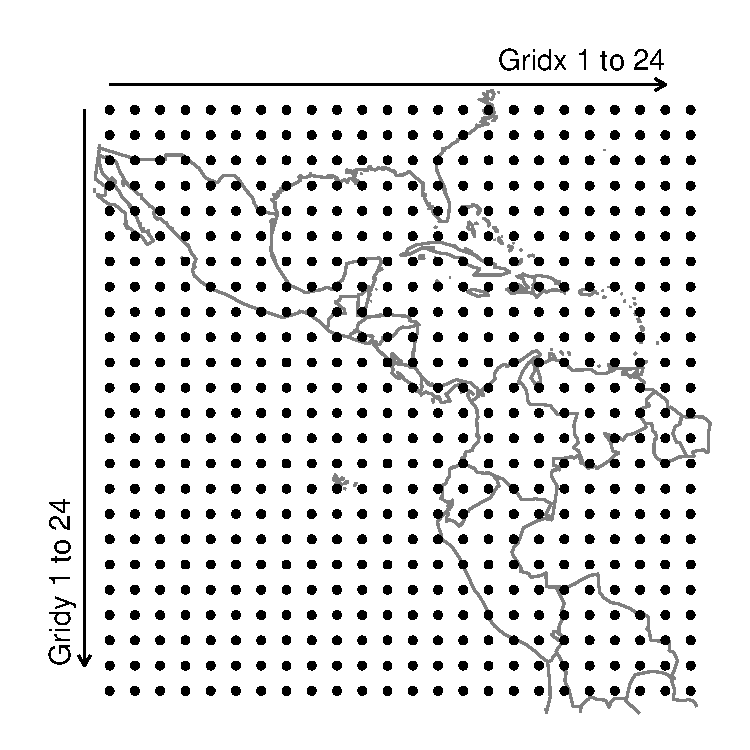
\includegraphics[width=\linewidth]{figure/nasa1}
\end{minipage}
\end{frame}

\begin{frame}[fragile]
\frametitle{What is a Time Series?}
\begin{minipage}{.42\linewidth}\footnotesize
\begin{itemize}
\item For each location multiple measurements
\begin{knitrout}\tiny
\definecolor{shadecolor}{rgb}{1, 1, 1}\color{fgcolor}\begin{kframe}
\begin{alltt}
\hlkwd{qplot}\hlstd{(TimeIndx, ts,} \hlkwc{geom}\hlstd{=}\hlstr{"point"}\hlstd{,}
      \hlkwc{data}\hlstd{=}\hlkwd{subset}\hlstd{(nasa, (Gridx}\hlopt{==}\hlnum{1}\hlstd{)}\hlopt{&}
                    \hlstd{(Gridy}\hlopt{==}\hlnum{1}\hlstd{)))}
\end{alltt}
\end{kframe}
\end{knitrout}
\item connected by a line
\begin{knitrout}\tiny
\definecolor{shadecolor}{rgb}{1, 1, 1}\color{fgcolor}\begin{kframe}
\begin{alltt}
\hlkwd{qplot}\hlstd{(TimeIndx, ts,} \hlkwc{geom}\hlstd{=}\hlstr{"line"}\hlstd{,}
      \hlkwc{data}\hlstd{=}\hlkwd{subset}\hlstd{(nasa, (Gridx}\hlopt{==}\hlnum{1}\hlstd{)}\hlopt{&}
                    \hlstd{(Gridy}\hlopt{==}\hlnum{1}\hlstd{)))}
\end{alltt}
\end{kframe}
\end{knitrout}
\item but only connect the right points
\begin{knitrout}\tiny
\definecolor{shadecolor}{rgb}{1, 1, 1}\color{fgcolor}\begin{kframe}
\begin{alltt}
\hlkwd{qplot}\hlstd{(TimeIndx, ts,} \hlkwc{geom}\hlstd{=}\hlstr{"line"}\hlstd{,}
      \hlkwc{data}\hlstd{=}\hlkwd{subset}\hlstd{(nasa, (Gridx}\hlopt{==}\hlnum{1}\hlstd{)}\hlopt{&}
              \hlstd{(Gridy}\hlopt\hlkwd{c}\hlstd{(}\hlnum{1}\hlstd{,}\hlnum{15}\hlstd{))),}
      \hlkwc{group}\hlstd{=Gridy)}
\end{alltt}
\end{kframe}
\end{knitrout}
\end{itemize}
\end{minipage}\hfill\begin{minipage}{.55\linewidth}
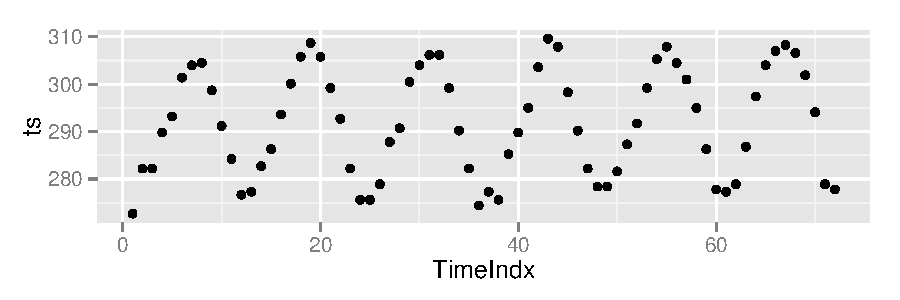
\includegraphics[width=\linewidth]{figure/tsplot1}\\
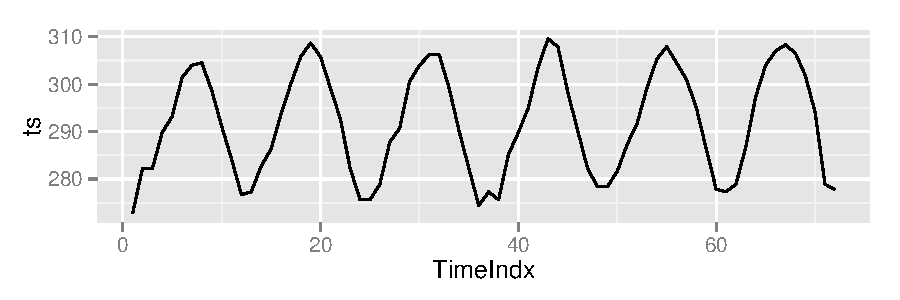
\includegraphics[width=\linewidth]{figure/tsplot2}\\
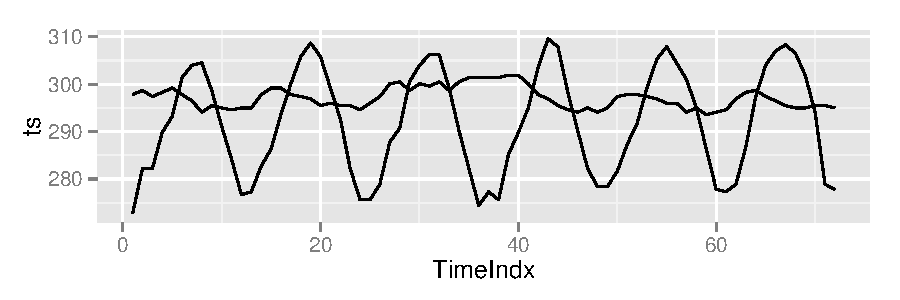
\includegraphics[width=\linewidth]{figure/tsplot3}
\end{minipage}
\end{frame}

\begin{frame}
\frametitle{Your Turn}
\begin{itemize}
\item Get a subset of locations, plot a time series for pressure for each location. \\\medskip{\footnotesize What is the general pattern?}\medskip
\item For all locations, draw individual time series for pressure.\\\medskip{\footnotesize What do you expect? Are there surprising values? Which are they?}\medskip
\item Introduce a Date (Year + Month) to the nasa data and change the pressure time series plot accordingly.
\end{itemize}
\end{frame}

\end{document}
